% 4

\chapter{Sviluppo}

Quando si vuole sviluppare un’applicazione desktop la prima cosa a cui si pensa è per quale sistema operativo svilupparla, quale linguaggio usare ed opzionalmente a quale base dati si ha bisogno di connettersi.
In questo caso la scelta è caduta su Electron, un framework Open Source sviluppato dal team di GitHub che permette lo sviluppo di app cross platform utilizzando il medesimo approccio di Apache Cordova, ovvero attraverso JavaScript, HTML, e CSS.
Si tratta di un modulo Npm, quindi eredita tutte le API e le funzionalità di Node.js.
\\
Il vero potenziale di Electron è dato dal fatto che si può costruire una desktop app utilizzando qualsiasi libreria scritta in Node.js, rendendolo di fatto uno strumento molto potente anche per interagire con il sistema operativo.
\\
Nello specifico dello sviluppo del sofware, si possono distinguere tre specifiche aree:
\begin{itemize}
	\item Front-End, comprende tutto ciò che riguarda l'interfaccia utente, quindi come presentare i dati passati dal Back-End, la grafica, il template, il typewriting, l’accessibilità e l’usabilità.
	\item Back-End, comprende tutto ciò che riguarda lo sviluppo della logica del software, ovvero cosa fare con i dati, come trattare quelli ricevuti, cosa restituire all'utente.
	\item Packaging dell'App, la creazione del prodotto finale, ovvero il software in versione eseguibile per tutte le tipologie di piattaforme di elaborazione.
\end{itemize}


% 4.1

\section{Sviluppo del Front-End}

Per lo sviluppo di un interfaccia utente efficace si deve tener conto di due aspetti oltre a quello tecnico, che sono:
\begin{itemize}
\item Accessibilità
\item Usabilità
\end{itemize}

In generale i requisiti di accessibilità sono i seguenti:
\begin{itemize}
    \item Alternative testuali, obbligatorie per tutte i contenuti non testuali (come immagini, filmati e audio);
    \item Adattabilità, cioè prevedere che i contenuti si adattino a diversi layout in base alla grandezza e al formato dello schermo utente (responsive web design);
    \item Distinguibile, rendere più semplice agli utenti la visione e l'ascolto dei contenuti, separando i contenuti in primo piano dallo sfondo;
    \item Accessibile da tastiera, cioè garantire una buona navigabilità prevedendo un percorso di TAB;
    \item Colori, il contrasto tra le scritte e lo sfondo deve essere chiaro, ma non si devono usare colori discordanti tra loro o lampeggianti che possano causare crisi epilettiche;
    \item Navigabile, fornire una struttura del sito chiara, dove l'utente possa orientarsi e raggiungire qualsiasi sezione attraverso links;
    \item Assistenza per l'inserimento, fornire gli aiuti e le spiegazioni necessarie affinché l'utente sia in grado di compilare correttamente le form del sito;
    \item Compatibilità, il sito deve essere accessibile da tutte le piattaforme e deve utilizzare tecnologie standard.
\end{itemize}


L'\textbf{usabilità} è un approccio alla progettazione volto a rendere l'interazione tra il prodotto e l'utente migliore sotto i seguenti aspetti:
\begin{itemize}
    \item Efficacia, cioè permettere agli utenti di raggiungere i loro obiettivi in maniera precisa e completa;
    \item Efficienza, cioè l'ottimizzazione delle risorse impiegate;
    \item Soddisfazione, come libertà dal disagio e attitudine positiva con cui gli utenti raggiungono specifici obiettivi attraverso l’uso del prodotto.
\end{itemize}
L'usabilità invece si pone i seguenti obiettivi:
\begin{itemize}
    \item Presentare l'informazione all'utente in modo chiaro e conciso, evitando termini tecnici o specialistici;
    \item Semplificare la struttura del compito;
    \item Offrire all'utente le scelte corrette, in una maniera che risulti ovvia;
    \item Organizzare ogni pagina in modo che l'utente riconosca la posizione e le azioni da compiere;
    \item Eliminare ogni ambiguità relativa alle conseguenze di un'azione (es. fare clic su cancella/rimuovi/compra);
    \item Mettere la cosa più importante nella posizione giusta della struttura;
    \item Fare in modo che l'utente abbia un rapido feedback ad ogni azione compiuta, ad esempio la comparsa di un messaggio di successo o errore all'invio di dati con una form;
    \item Rendere la grafica accattivante ed interessante dal punto di vista visivo attraverso l'uso di diagrammi, tabelle, sezioni informative e coordinando bene i colori;
    \item Ridurre gli sforzi cognitivi dell'utente.
\end{itemize}
In generale cercare di rendere il sistema il più semplice possibile da usare, in modo da ridurre al minimo gli sforzi sull'utilizzo del mezzo.

% 4.1.1

\subsection{Tecnologie usate nello sviluppo del front-end}

Mentre per lo sviluppo del back-end abbiamo a disposizione una gran quantità di tecnologie concorrenti per svolgere lo stesso compito, per il front-end le tecnologie di base sono sempre le stesse: \Gls{html}, \Gls{css}, JavaScript e Jquery.
\\
\textbf{\Gls{html}} è un linguaggio di markup che serve per descrivere le modalità di impaginazione, formattazione o visualizzazione grafica (layout) del contenuto, testuale e non, di una pagina web.
Per specificare tali disposizioni e proprietà si utilizzano specifici marcatori chiamati “tag“, i quali delimitano gli elementi stessi (ad esempio \textless p\textgreater  per i paragrafi, \textless h1\textgreater  per un titolo di primo livello, \textless  address\textgreater  per informazioni relative ad un indirizzo, etc.).\\
La versione più recente è chiamata HTML 5 e rispetto alle versioni precedenti ha l'aggiunta di alcuni tag per gli elementi mutlimediali, una rivisitazione delle regole di strutturazione del testo riguardante sezioni, paragrafi e capitoli, il miglioramento i controlli di input per le form, il controllo della geolocalizzazione e l'intruduzione dello Web Storage come alternativa ai cookies.
\\
\textbf{\Gls{css}} descrive come devono essere visualizzati gli elementi in una pagina web. A differenza dell'\Gls{html} che è usato per strutturare un documento (definendo cose come titoli e paragrafi e permettendo di incorporare immagini, video e altri media), il \Gls{css} passa attraverso e specifica i layout di stile della pagina del documento, i colori e i caratteri. Il codice \Gls{css} può essere esterno, interno o in linea, nel software realizzato la scelta è stata quella di separare in due file distinti il codice \Gls{html} e il codice \Gls{css}.

\begin{figure}[H]
    \centering
    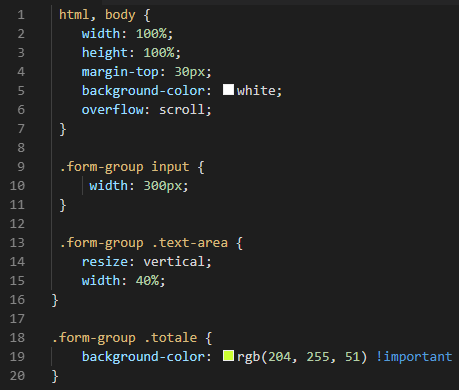
\includegraphics{css.png}
    \caption{esempio di utilizzo di css nel software}
    \label{fig:css}
\end{figure}

\textbf{JavaScript} è rimasto confinato per quasi 2 decenni nel browser, prima di diventare un linguaggio di programmazione anche per lo sviluppo del backend con la nascita di Node.js. Lato front-end comunque, Javascript viene utilizzato principalmente per aggiungere effetti dinamici interattivi basati su eventi, come il click di un bottone, la selezione di una voce da una tendina, la pressione di un tasto o il caricamento di una pagina, ed è comunque consigliato per aumentare l'esperienza utente. 

\begin{figure}[H]
    \centering
    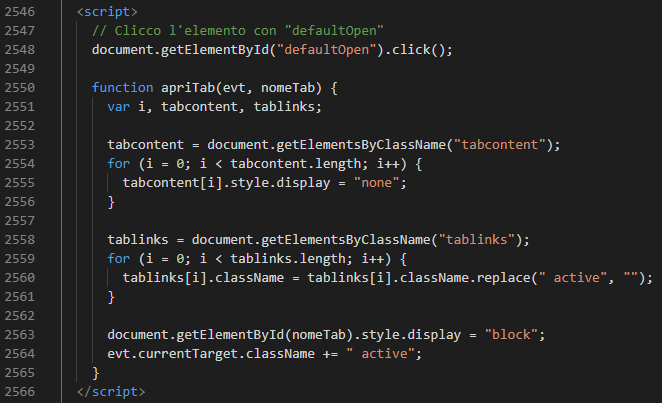
\includegraphics[scale=0.8]{javascript.png}
    \caption{javascript per selezione tab}
    \label{fig:javascript}
\end{figure}

Nella figura ~\ref{fig:javascript} viene mostrato un esempio di come Javascript venga utilizzato lato front-end, nel caso specifico per la selezione e la visualizzazione delle tab del software. \\


\textbf{jQuery} è una libreria JavaScript che contiene tutto il necessario per creare interazioni avanzate per le pagine web, con lo scopo di semplificare la selezione, la gestione e la manipolazione degli eventi, mantenendo però anche la possibilità di utilizzare il linguaggio nella vecchia maniera. \\
L'uso di jQuery non aggiunge quindi nessuna funzionalità, rende solamente più semplice l'utilizzo del linguaggio e quindi più elevata la produttività del programmatore, non a caso il suo motto è "Write less, do more".

\begin{figure}[H]
    \centering
    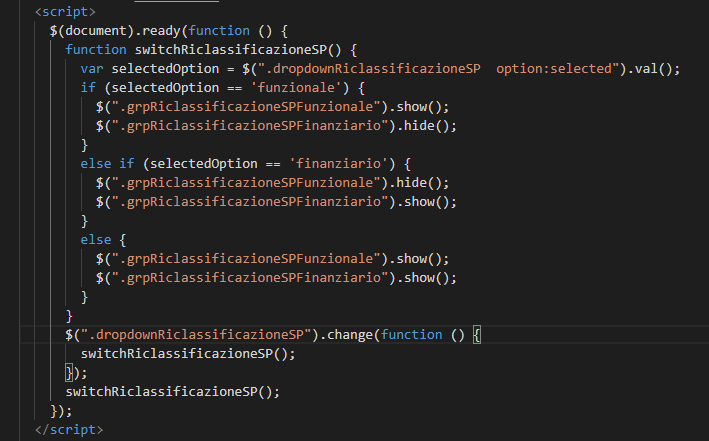
\includegraphics[scale=0.8]{jquery1.png}
    \caption{jquery per scelta tipologia riclassificazione}
    \label{fig:jquery1}
\end{figure}

\begin{figure}[H]
    \centering
    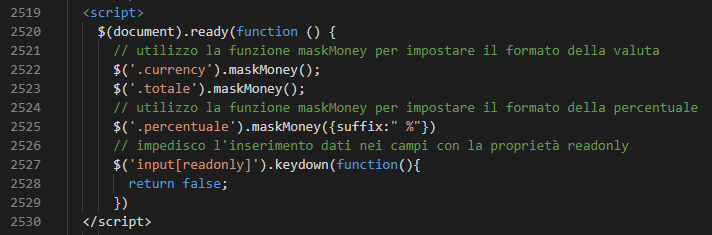
\includegraphics[scale=0.8]{jquery2.png}
    \caption{jquery per maskmoney}
    \label{fig:jquery2}
\end{figure}

Jquery nell'applicazione realizzata, come si può vedere nelle figure ~\ref{fig:jquery1} e ~\ref{fig:jquery2}, viene utilizzato nello sviluppo lato back-end per la selezione della tipologia di riclassificazione, e attraverso l'utilizzo dei selettori per richiamare la funzione MaskMoney, importata da una libreria esterna, la quale permette la formattazione dei valori nell'interfaccia, a seconda della tipologia di dato (valuta o percentuale).

% 4.2

\newpage

\section{Sviluppo del Back-End}

Nella struttura di un app basata su Electron, bisogna discutere di due tipi di processo esistenti:
\begin{itemize}
	\item  il processo chiamato \textbf{main} che esegue lo script indicato nel file package.json è il processo principale. Lo script che viene eseguito nel processo principale può visualizzare una \Gls{gui} tramite la creazione di pagine web. Il processo principale crea pagine web mediante la creazione di istanze di BrowserWindow, dove vengono eseguite nel proprio processo di rendering. Quando viene eliminata un'istanza di BrowserWindow, il processo di rendering corrispondente viene anch'esso terminato. Il processo principale quindi, gestisce tutte le pagine web e il corrispondente processo di rendering.
	\item il processo di \textbf{rendering}, invece è il processo che gestisce ogni pagina web, visualizzata tramite Chromium con la sua architettura multi-processo, tale processo è isolato e può occuparsi solo delle pagine web in esecuzione in esso.
	Pertanto nelle pagine web chiamare le API dell'interfaccia grafica nativa non è consentito perché la gestione delle risorse di sistema nelle pagine web è molto pericolosa ed è facile perdere risorse. Se si desidera eseguire operazioni di \Gls{gui} in una pagina web, il processo di rendering della pagina web deve comunicare con il processo principale per richiedere che il processo principale esegua tali operazioni.
\end{itemize}

\begin{figure}[H]
    \centering
    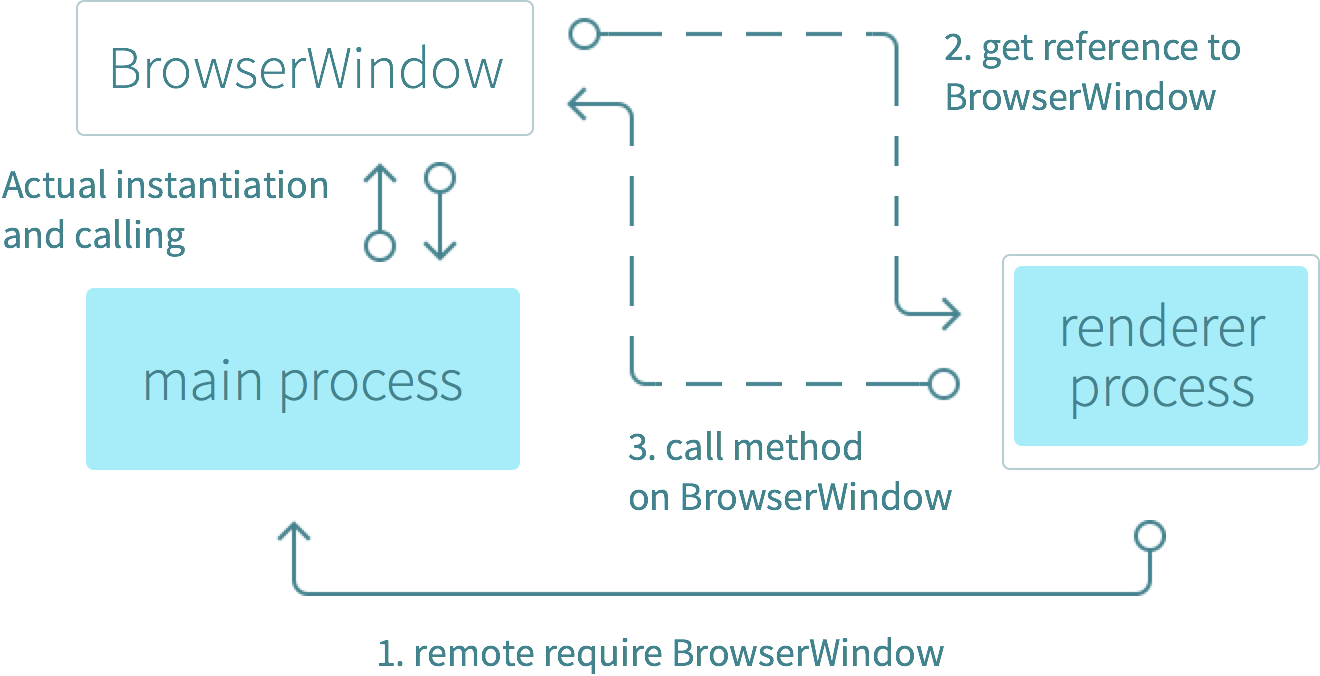
\includegraphics[scale=0.25]{electron-architecture.png}
    \caption{Electron - Architettura di un app}
    \label{fig:ElectronArch}
\end{figure}

% 4.2.1

\subsection{Utilizzo delle API Electron}

Electron offre una serie di API che supportano lo sviluppo di un'applicazione desktop sia nel processo principale che nel processo di rendering. In entrambi i processi, devi accedere alle API di Electron richiedendo il relativo modulo incluso:

\begin{figure}[H]
    \centering
    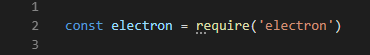
\includegraphics{apiElectron.png}
    \caption{importazione API Electron}
    \label{fig:ApiElectron}
\end{figure}

A tutte le API Electron viene assegnato un tipo di processo. Molti di essi possono essere utilizzati solo dal main, alcuni solo da un processo di rendering, alcuni da entrambi. Ad esempio, una finestra in Electron viene creata utilizzando la classe BrowserWindow, disponibile solo nel processo principale.

\begin{figure}[H]
    \centering
    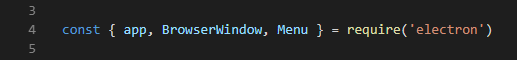
\includegraphics{browserWindow.png}
    \caption{importazione classe BrowserWindow}
    \label{fig:BrowserWindow}
\end{figure}

\begin{figure}[H]
    \centering
    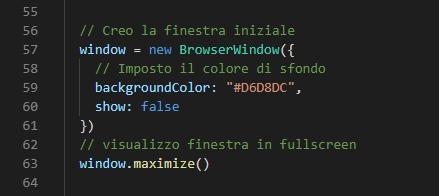
\includegraphics{browserWindow2.png}
    \caption{Creazione BrowserWindow}
    \label{fig:BrowserWindow2}
\end{figure}


% 4.2.2

\subsection {Apertura e salvataggio del progetto}

Durante l'utilizzo del software l'utente deve avere la possibilità attraverso una funzione apposita, di poter salvare un progetto in stato d'opera e/o di leggere un progetto precedentemente salvato.
Per la realizzazione di questa funzionalità, si è scelto di non utilizzare un database ma di un semplice salvataggio dei dati attraverso un file \Gls{json} nel file system della piattaforma di elaborazione in uso.
JSON è un modo per archiviare le informazioni in modo organizzato e di facile accesso per l'utilizzo delle stesse all'interno di una applicazione (web, mobile o di qualsiasi altro tipo).

\begin{figure}[H]
    \centering
    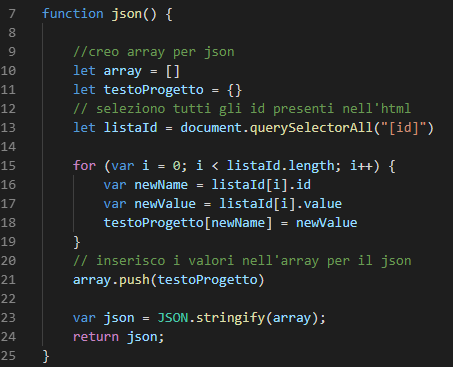
\includegraphics{json.png}
    \caption{Creazione Json}
    \label{fig:json}
\end{figure}

Nella figura ~\ref{fig:json} viene mostrata l'implementazione della funzione "json" per la creazione del file JSON contenente i valori inseriti nel progetto. Inizialmente, utilizzando la funzione querySelectorAll vengono selezionati tutti gli Id contenuti nell'html del main, successivamente, attraverso un ciclo for per l'iterazione degli stessi, vengono inseriti nell'array contenuto nel JSON.

\begin{figure}[H]
    \centering
    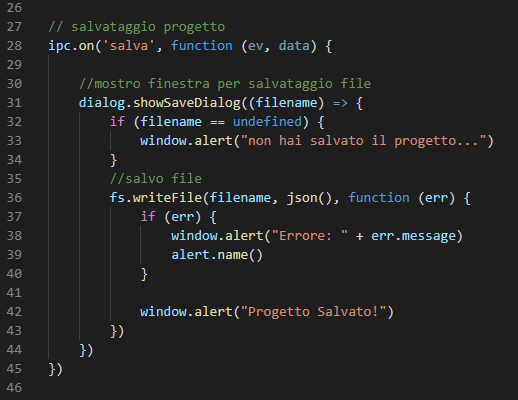
\includegraphics{salvataggio.png}
    \caption{funzione salvataggio}
    \label{fig:salvataggio}
\end{figure}

Electron per comunicare tra processi renderer e main, in entrambe le direzioni, utilizza la comunicazione interprocesso \Gls{ipc}.\\  Come mostrato nella figura ~\ref{fig:salvataggio} la funzione relativa al salvataggio del progetto viene richiamata tramite IPC al messaggio 'salva', e grazie all'utilizzo delle API di Node.js, viene creato all'interno del file system, il file JSON passato dalla funzione "json()" precedentemente illustrata.


% 4.2.3

\newpage

\subsection {Calcolo riclassificazioni e forecast}

Come già visto precedentemente, per l'analisi di bilancio di un'azienda spesso si utilizzano diverse tipologie di riclassificazione, sia per lo stato patrimoniale che per il conto economico. Nel software realizzato si è deciso di mettere a disposizione all'utente, per quanto riguarda lo stato patrimoniale la scelta tra la riclassificazione finanziario, funzionale o entrambe, mentre per il conto economico viene calcolata solo la riclassificazione al valore aggiunto.
Le riclassificazioni calcolate vengono poi usate per calcolare gli indici per il forecast per l'anno di riferimento del progetto.
Per il calcolo delle varie riclassificazioni e forecast sono state realizzate delle specifiche classi Javascript, in cui attraverso l'utilizzo di Jquery per l'acceso al \Gls{dom} e attraverso la funzione importata con la libreria del MaskMoney illustrata precedentemente, vengono applicate tutte le formule del caso.
Dove c'è la necessità di una sommatoria di più valori, ove possibile, è stato utilizzato l'attributo name del \Gls{dom} e attraverso un ciclo for calcolato il totale. Come in figura ~\ref{fig:riclassificazione}, dove viene mostrato l'esempio per il Totale patrimonio netto, calcolato prendendo tutti gli elementi che hannno l'attributo name all'interno dei vari tag impostato a SPFOPatrimonioNetto \\


\begin{figure}[H]
    \centering
    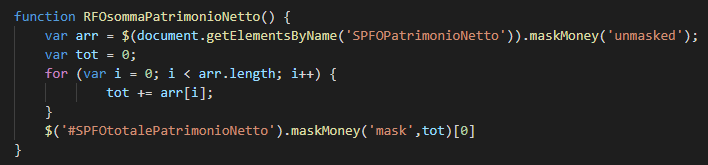
\includegraphics[scale=0.8]{riclassificazione.png}
    \caption{for per somma riclassificazione}
    \label{fig:riclassificazione}
\end{figure}

\newpage

Altrimenti, come nel caso specifico del forecast, in cui non poteva essere usato l'attributo name, si fa riferimento all'attributo id. Un esempio in figura ~\ref{fig:forecast}

\begin{figure}[H]
    \centering
    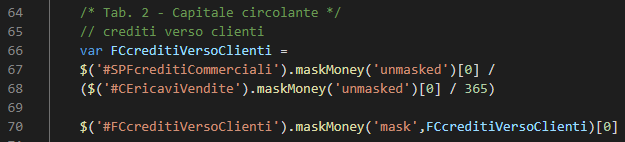
\includegraphics[scale=0.8]{forecast.png}
    \caption{esempio di calcolo per il forecast}
    \label{fig:forecast}
\end{figure}

% 4.2.4

\subsection {Creazione pdf}

Per la creazione di un report dei dati inseriti e calcolati, è stata utilizzata la comunicazione interprocesso \Gls{ipc}. 

\begin{figure}[H]
    \centering
    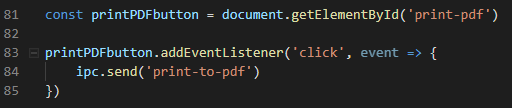
\includegraphics{pdf1.png}
    \caption{input da pulsante}
    \label{fig:pdf1}
\end{figure}

Nel processo di rendering viene impostato un handler atrraverso la funzione addEventListener() per poter inviare al processo principale il messaggio 'print-to-pdf', non appena l'utente che utilizza il sistema clicca sul bottone per la stampa del pdf, come da figura ~\ref{fig:pdf1}

\begin{figure}[H]
    \centering
    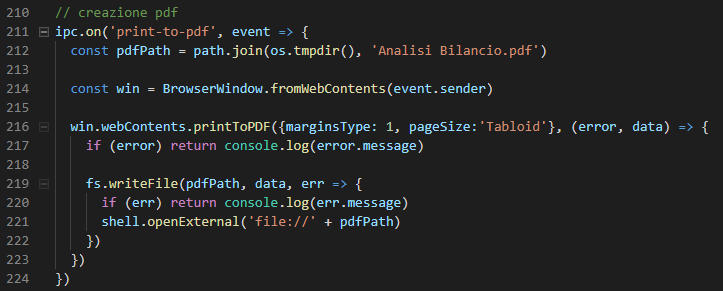
\includegraphics[scale=0.8]{pdf2.png}
    \caption{creazione e apertura del pdf}
    \label{fig:pdf2}
\end{figure}

Il processo principale, ricevuto il messaggio 'print-to-pdf' dal processo render, genera il file pdf in un percorso temporaneo del sistema operativo in uso e lo apre non appena creato.

\begin{figure}[H]
    \centering
    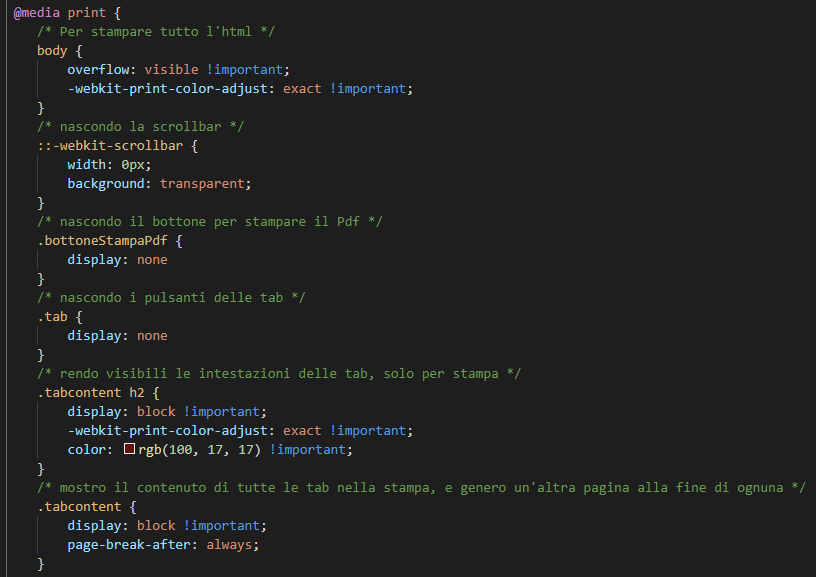
\includegraphics[scale=0.7]{pdfCss.png}
    \caption{specifica Css per stampa documenti}
    \label{fig:pdfCss}
\end{figure}

Il pdf viene generato grazie all'aiuto della specifica \Gls{css} per la stampa dei documenti, mostrato in, dove tra le varie istruzioni, vengono nascosti alcune parti del front end, come la scrollbar o i pulsanti delle tab, per mostrare invece tutta la parte del frontespizio del pdf generato.


% 4.3

\newpage

\section{Packaging dell'applicazione}

L'imballaggio e la distribuzione di app sono parte integrante del processo di sviluppo di un'applicazione desktop, poiché Electron è un framework di sviluppo di applicazioni desktop multipiattaforma, anche l'imballaggio e la distribuzione di app per tutte le piattaforme dovrebbero essere un'esperienza senza soluzione di continuità.
Per questo scopo, è stato utilizzato uno strumento da riga di comando e una libreria Node.js che ci consente di confezionare e distribuire la nostra app Electron con pacchetti specifici del sistema operativo (.app, .exe, ecc.), tramite \Gls{cli}, chiamato Electron Packager. Electron Packager funziona per le seguenti piattaforme:
\begin{itemize}
	\item Windows (32/64 bit)
	\item OS X (noto anche come macOS)
	\item Linux (x86/ x86-64)
\end{itemize}


Per utilizzare il pacchetto è necessario prima installarlo, usando all'interno della cartella del proprio progetto la riga di comando: "npm install electron-packager --save-dev".
Per creare il risultato finale del software il comando da eseguire è "electron-packager \textless dir\textgreater  \textless nomeApp\textgreater  --platform= \textless platform\textgreater  --arch= \textless arch\textgreater" dove:
\begin{itemize}
	\item  \textless dir\textgreater  è il percorso dove viene creata l'applicazione
	\item  \textless nomeApp\textgreater  è il nome dell'applicazione
	\item  \textless platform\textgreater  è la piattaforma di destinazione
	\item  \textless arch\textgreater  è la specifica dell'architettura del sistema operativo
\end{itemize}




